\documentclass[wide,a4paper,titlepage,12pt] {article}
\usepackage{polski}
\usepackage[utf8]{inputenc}
\usepackage{listings}
\usepackage{slashbox}
\usepackage[table]{xcolor}
\usepackage{graphicx,pdflscape}
\usepackage{placeins}

\title{Układy cyfrowe i systemy wbudowane}
\author{Tymon Tobolski (181037)\\ Jacek Wieczorek (181043)}

% Title page layout (fold)
\makeatletter
\renewcommand{\maketitle}{
\begin{titlepage}
  \begin{center}
    \vspace*{3cm}
    \LARGE \@title \par
    \vspace{2cm}
    \textit{\small Autor:}\par
    \normalsize \@author\par \normalsize
    \vspace{3cm}
    \textit{\small Prowadzący:}\par
    Dr inż. Jarosław Sugier \par
    \vspace{2cm}
    Wydział Elektroniki\\ III rok\\ Pn 14.15 - 16.00\par
    \vspace{4cm}
    \small \@date
  \end{center}
\end{titlepage}
}
\makeatother

\begin{document}
\maketitle
  \section{Zadanie nr 1}
  Celem zadania było stworzenie układu generującego sygnał prostokątny o zadanym przebiegu.
  Układ składał się z dwóch podukładów: licznika "0-7" oraz dekodera "1 z 8".
  Oba podukłady zostały zaimplementowane jako osobne urządzenia, a następnie użyte w głównym układzie.

  \begin{figure}[htbp]
    \begin{center}
      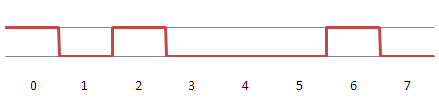
\includegraphics[scale=0.6]{syg.png}
      \caption{Przebieg sygnału}
     \end{center}
  \end{figure}

  \subsection{Licznik}
  Licznik działający asynchronicznie został stworzony za pomocą trzech przerzutników typu T połączonych kaskadowo. Pierwszy przerzutnik był sterowany zegarem, pozostałe były aktywowane opadającym zboczem swojego poprzednika.

  \begin{figure}[htbp]
    \begin{center}
      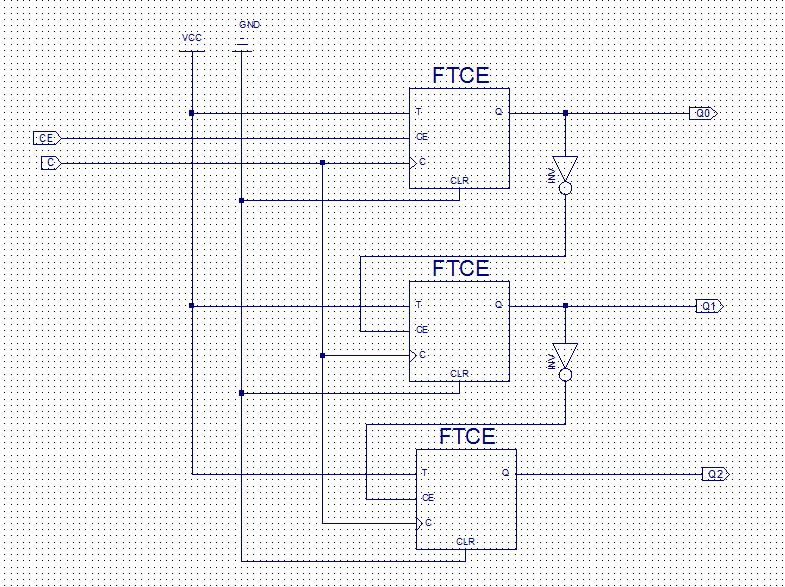
\includegraphics[scale=0.6]{licznik_asynch.png}
      \caption{Schemat licznika asynchronicznego}
     \end{center}
  \end{figure}

  \subsection{Dekoder}
  Dekoder sygnału 3-bitowego na sygnał 8-bitowy został utworzony z 8 po trójnych brame AND z zanegowanymi odpowiednimi wejściami.

  \begin{figure}[htbp]
    \begin{center}
      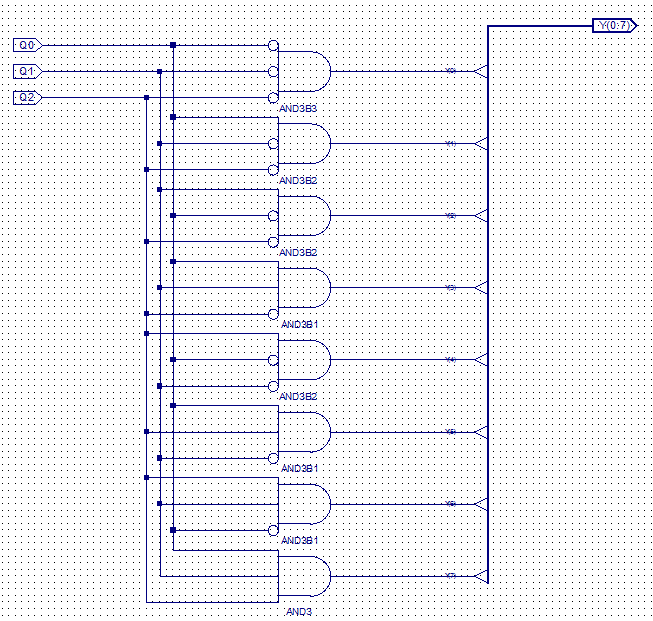
\includegraphics[scale=0.6]{dekoder.png}
      \caption{Schemat dekodera}
     \end{center}
  \end{figure}

\end{document}



